\documentclass[11pt]{article}

\usepackage[margin=1in]{geometry}
\usepackage{amsmath, amssymb}
\usepackage{booktabs}
\usepackage{graphicx}
\usepackage{hyperref}
\usepackage{caption}
\usepackage{subcaption}
\usepackage{microtype}

\title{Frozen Islands and Small-World Mixing in Lattice Gambler's Ruin}
\author{Exploratory simulation note}
\date{\today}

\begin{document}
\maketitle

\begin{abstract}
We study a square-lattice version of multiplayer gambler's ruin in which wealth is conserved, neighboring active sites exchange one unit of wealth at random, and dead sites become permanent barriers. This minor local-interaction change turns the classical absorption story into a spatial pattern-formation problem. Instead of a single eventual winner, the system generically freezes into many isolated active remnants separated by dead zones. We quantify the resulting patterns with active density, cluster counts, cluster-size distributions, initial wealth concentration, and a small-world nonlocality scan. The main empirical finding is sharp and useful: adding random nonlocal edges does not force global absorption in the tested $N=100$, initial-wealth $10$ regime. It prolongs competition, lowers the final density of surviving active sites, and leaves a frozen dust of isolated survivors.
\end{abstract}

\section{Premise}

Classical gambler's ruin is usually non-spatial. If all players can eventually interact, finite total wealth and unbiased exchanges imply eventual absorption by one surviving player. The lattice model changes only the interaction graph. Sites occupy an $N \times N$ grid; in each round, active neighboring pairs are matched, one endpoint wins one dollar, and the other loses one dollar. A site with zero wealth is dead. In this version, dead sites remain barriers: they do not play and they do not transmit interactions.

This rule is deliberately simple. It asks whether ruin dynamics can create geometric structure without any explicit growth law, surface tension, fitness, or external field. The answer is yes. Death creates holes; holes break connectivity; broken connectivity creates frozen islands.

\section{Model}

Let $A_i(t) \in \mathbb{Z}_{\ge 0}$ denote the wealth at lattice site $i$ at time $t$. Total wealth is conserved:
\[
  \sum_i A_i(t) = W.
\]
For a graph $G=(V,E)$, only edges $(i,j)\in E$ with $A_i(t)>0$ and $A_j(t)>0$ are playable. In each round, we greedily form a random matching from the currently active edges, and every matched pair performs
\[
  (A_i,A_j) \mapsto (A_i+1,A_j-1)
  \quad\text{or}\quad
  (A_i-1,A_j+1)
\]
with equal probability. The process stops when no active--active edge remains. This stopping state may contain many active sites, but every active site is isolated from every other active site in the interaction graph.

For the base lattice, $G$ is the nearest-neighbor von Neumann square lattice. For the small-world experiment, we keep all local edges and add long-range edges as follows: for each vertex, with probability $p$, choose one uniformly random non-neighbor and add an undirected edge.

\section{Measurements}

We use four families of measurements.

\paragraph{Spatial state.}
Heatmaps show initial wealth, final wealth, and final active sites. These are the most direct pattern-formation outputs.

\paragraph{Cluster structure.}
Clusters are connected components of active sites under the chosen lattice neighborhood. A frozen final state under purely local interactions can still have clusters larger than one if the run is capped before full freezing; in a fully frozen state on the full interaction graph, no active--active edge remains.

\paragraph{Initial concentration.}
Initial wealth concentration is summarized by the Herfindahl--Hirschman index
\[
  \mathrm{HHI}(A(0)) = \sum_i \left(\frac{A_i(0)}{W}\right)^2,
\]
and by $1-\mathrm{HHI}$ as the corresponding diversity measure. HHI is the natural bifurcation parameter because it directly measures how concentrated the initial field is.

\paragraph{Nonlocality.}
For the small-world scan we record freeze time, active density, cluster count, largest cluster fraction, and the realized fraction of matches that used nonlocal edges.

\section{Experiments}

All headline spatial experiments used $N=100$. The random-field lattice run used von Neumann neighborhoods, random-gamma initial wealth with heterogeneity parameter $5$, initial wealth scale $25$, ten simulations, and a $3000$-round observation horizon. The HHI bifurcation scan used ten simulations per target HHI value, $0.01 \leq \mathrm{HHI} \leq 0.50$, and a $1000$-round horizon for tractability. The small-world scan used uniform initial wealth $10$, seed $123$, ten simulations per $p$, and no round cap. The nonlocal probabilities ranged from $p=0.04$ to $p=0.90$ in steps of $0.02$.

\section{Results}

\subsection{Frozen Pattern Formation}

Figure~\ref{fig:heatmaps} shows the basic phenomenon. Wealth starts as a heterogeneous but fully active field. After many local exchanges, the final active set is sparse and fragmented. Dead zones are not passive bookkeeping; they are the mechanism that cuts the interaction graph.

\begin{figure}[ht]
  \centering
  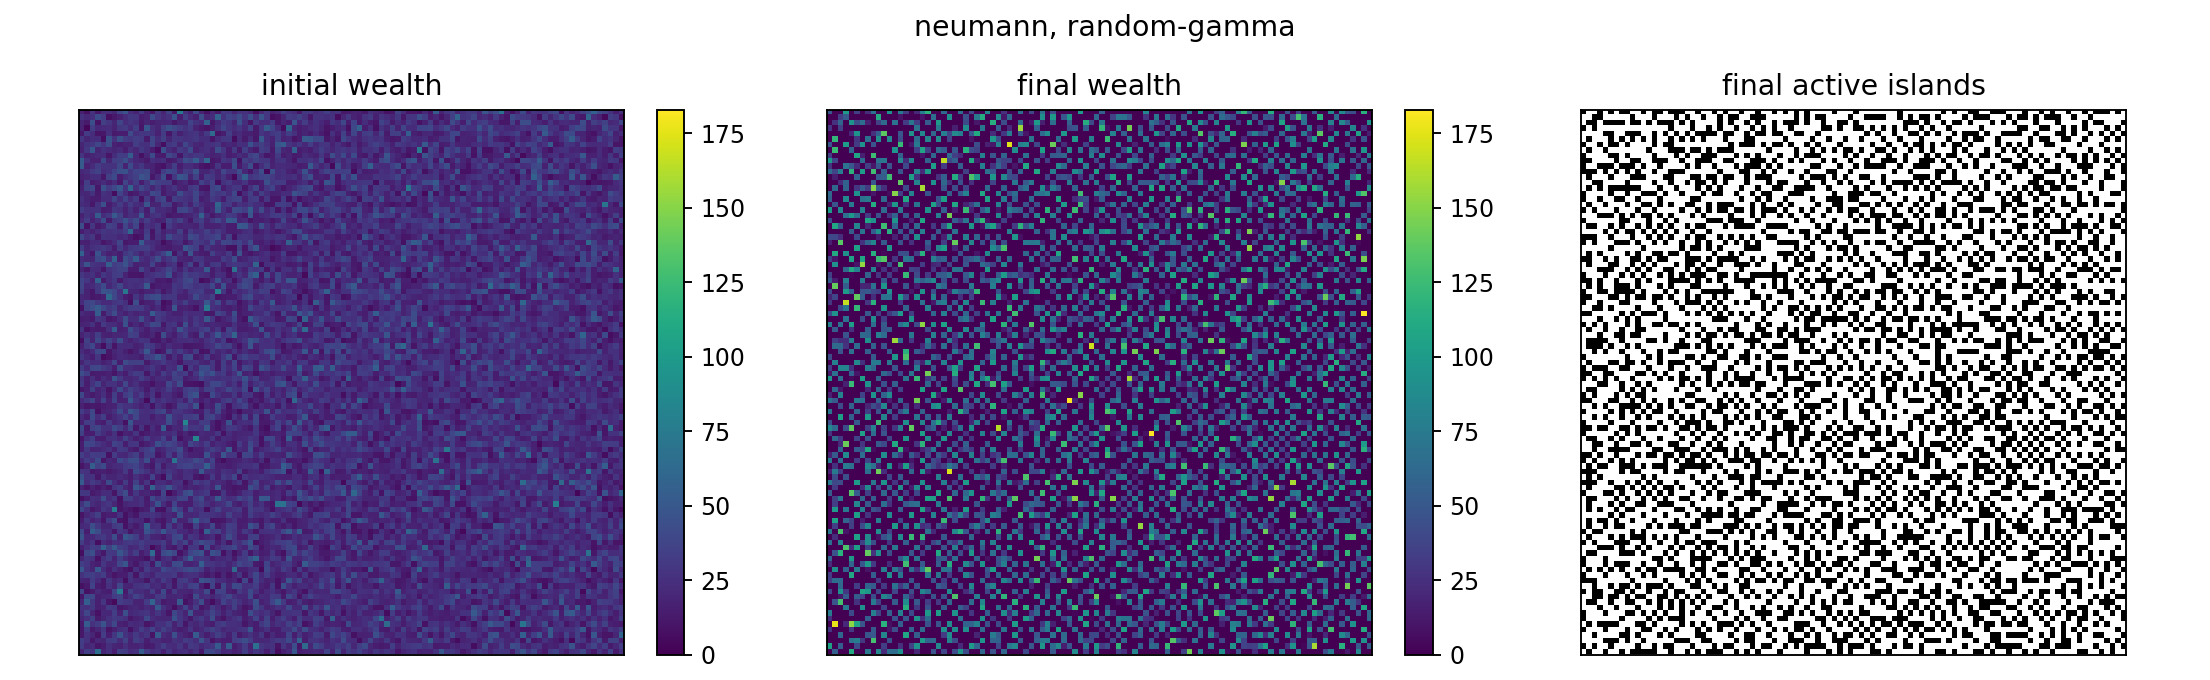
\includegraphics[width=0.96\linewidth]{figures/heatmaps_N100_gamma.png}
  \caption{Initial wealth, final wealth, and final active mask for a representative $N=100$ random-gamma lattice run. Dead sites create barriers and fragment the active set.}
  \label{fig:heatmaps}
\end{figure}

The final wealth histogram in Figure~\ref{fig:histogram} separates two facts: most sites become dead, while the remaining active sites carry larger wealth. This is exactly the conserved-wealth version of coarsening: mass concentrates, but spatial barriers prevent global coalescence.

\begin{figure}[ht]
  \centering
  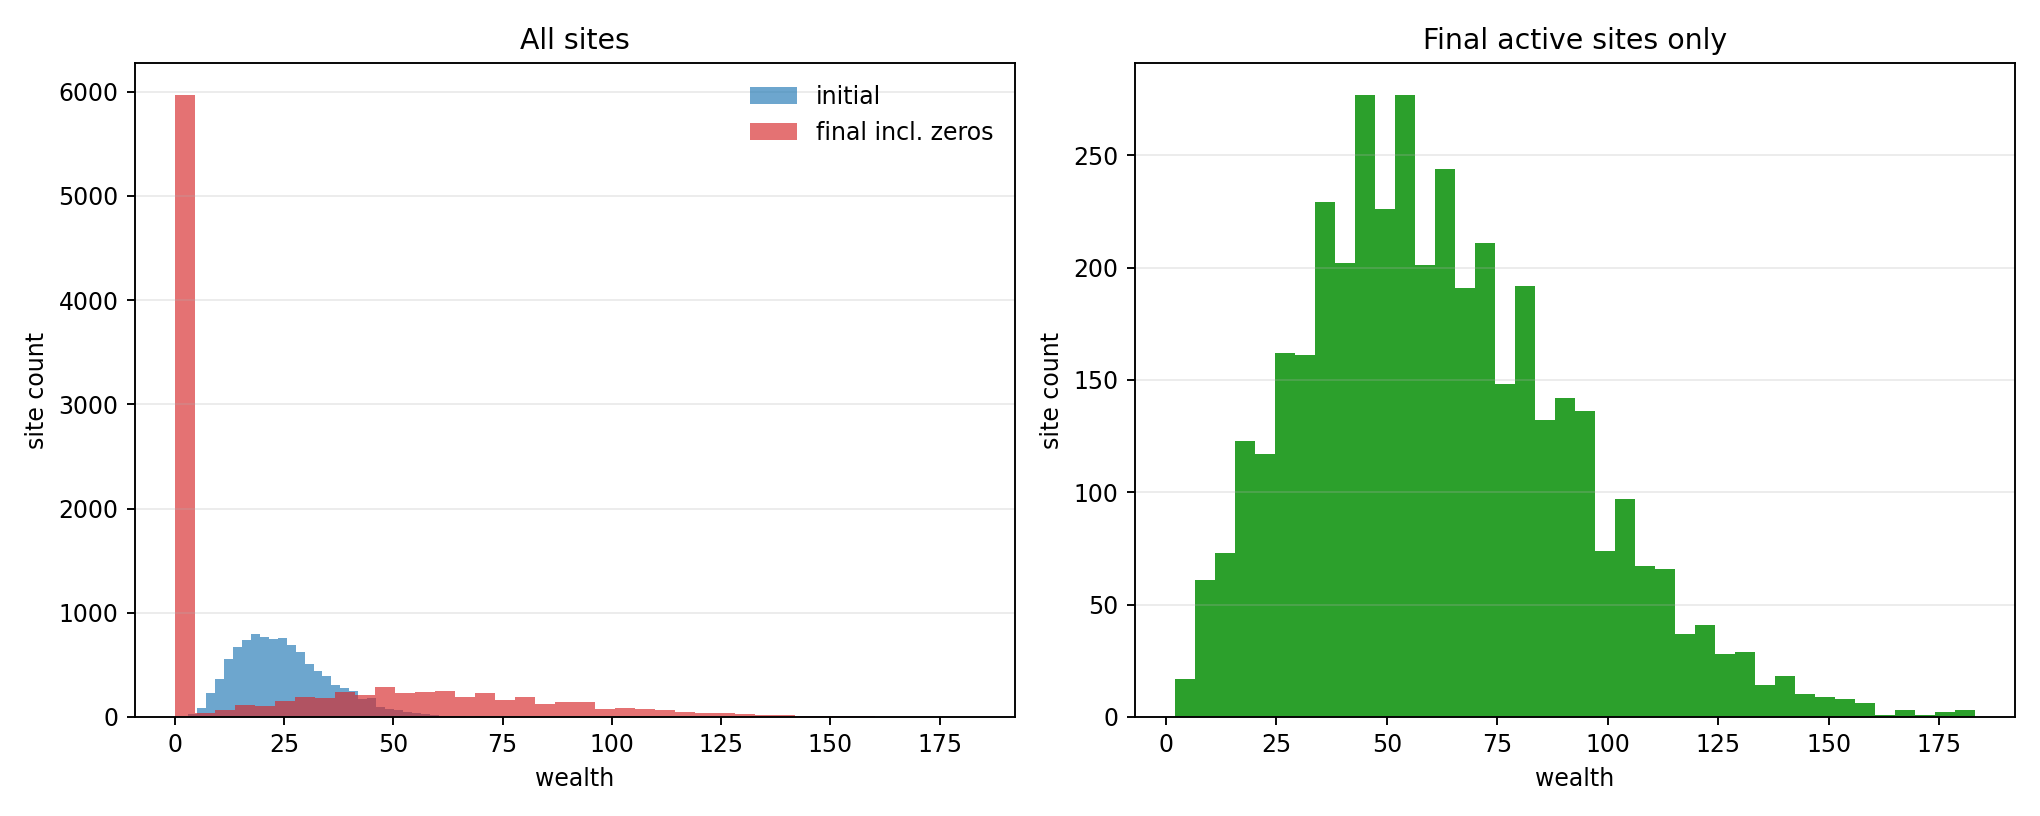
\includegraphics[width=0.82\linewidth]{figures/wealth_histogram_N100_gamma.png}
  \caption{Initial and final wealth histograms. The final distribution has a large atom at zero and a heavier active-site tail.}
  \label{fig:histogram}
\end{figure}

\subsection{Cluster Sizes}

The cluster-size diagnostic in Figure~\ref{fig:clusters} is useful, but it must be interpreted carefully. The log--log plot is not evidence of a clean power law. A single global fit is poor; the two-regime fit is more honest. Small components dominate, and large components are rare in this regime. The meaningful empirical point is not a universal exponent, but the presence of a broad, noisy component-size spectrum during finite-time coarsening.

\begin{figure}[ht]
  \centering
  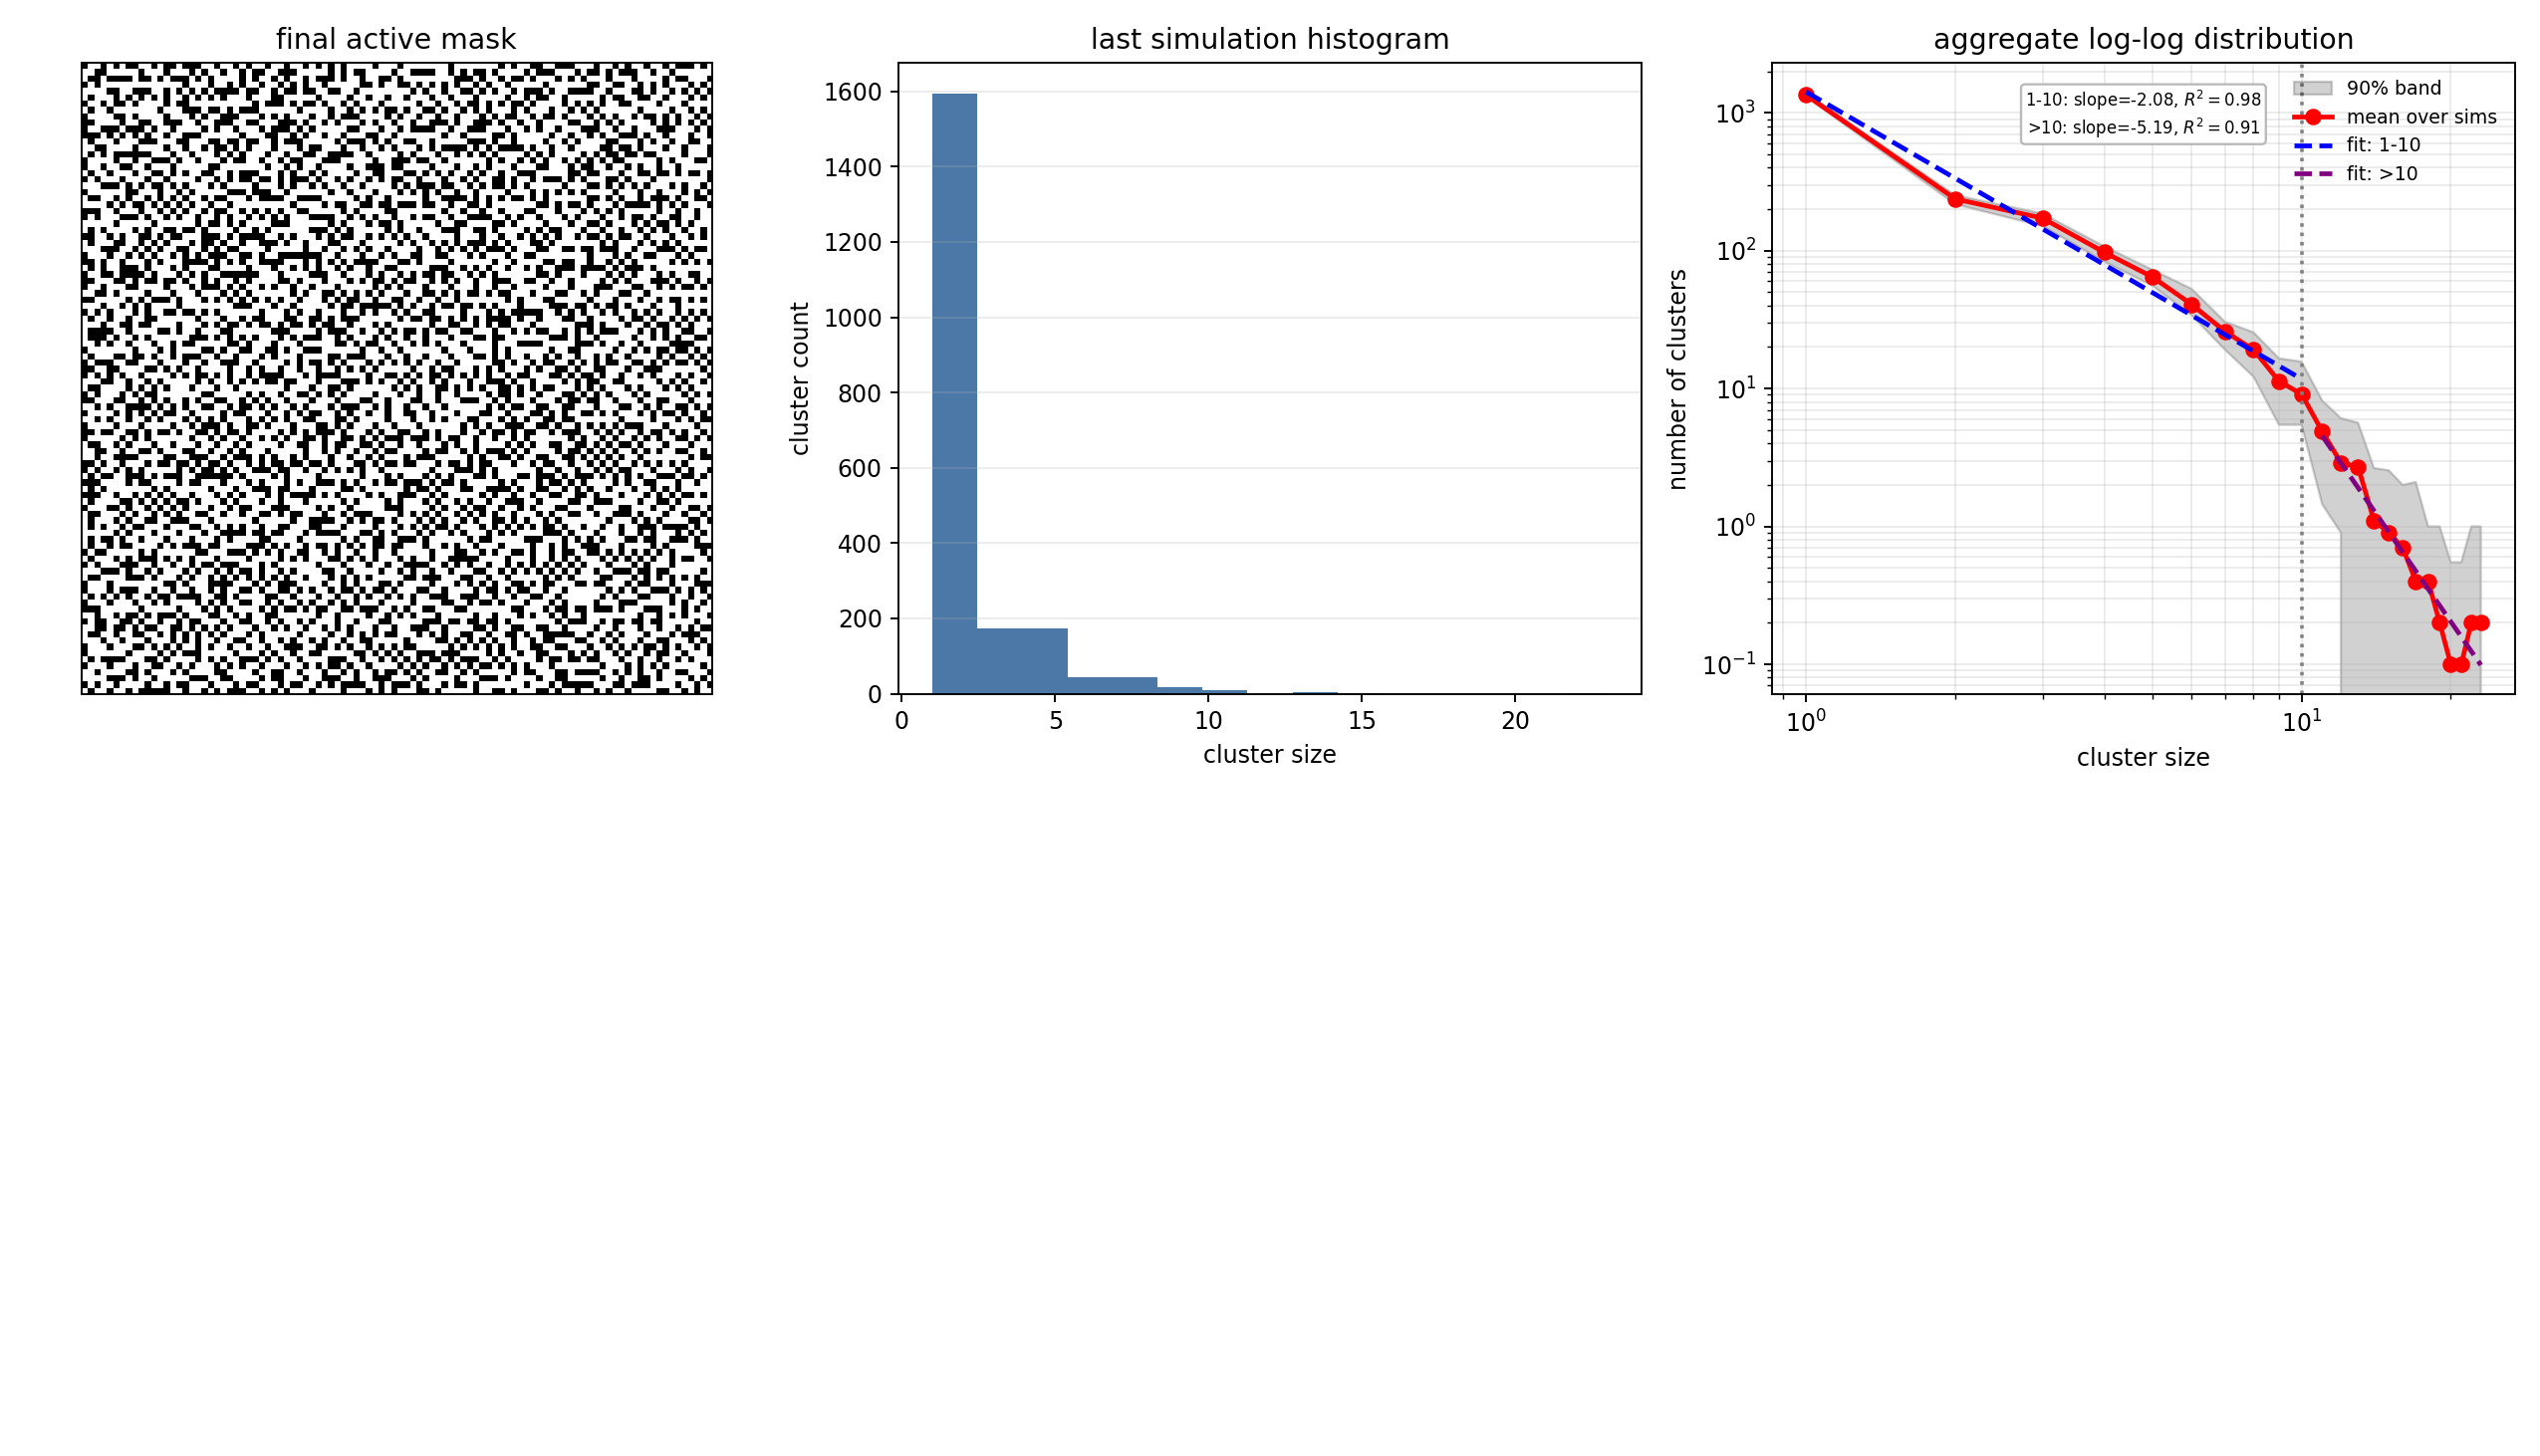
\includegraphics[width=0.96\linewidth]{figures/cluster_sizes_N100_gamma.png}
  \caption{Cluster-size summaries across ten $N=100$ random-gamma simulations. The aggregate log--log panel uses a 90\% band and separate small- and large-cluster fits.}
  \label{fig:clusters}
\end{figure}

\subsection{Initial HHI as a Bifurcation Parameter}

Figure~\ref{fig:hhi} supports the use of initial HHI as the right control variable. Low HHI corresponds to diffuse initial wealth; high HHI corresponds to concentrated initial wealth. Even with a capped horizon, the final active density, cluster count, largest-island fraction, and time-to-cap/freeze change systematically with measured initial HHI.

\begin{figure}[ht]
  \centering
  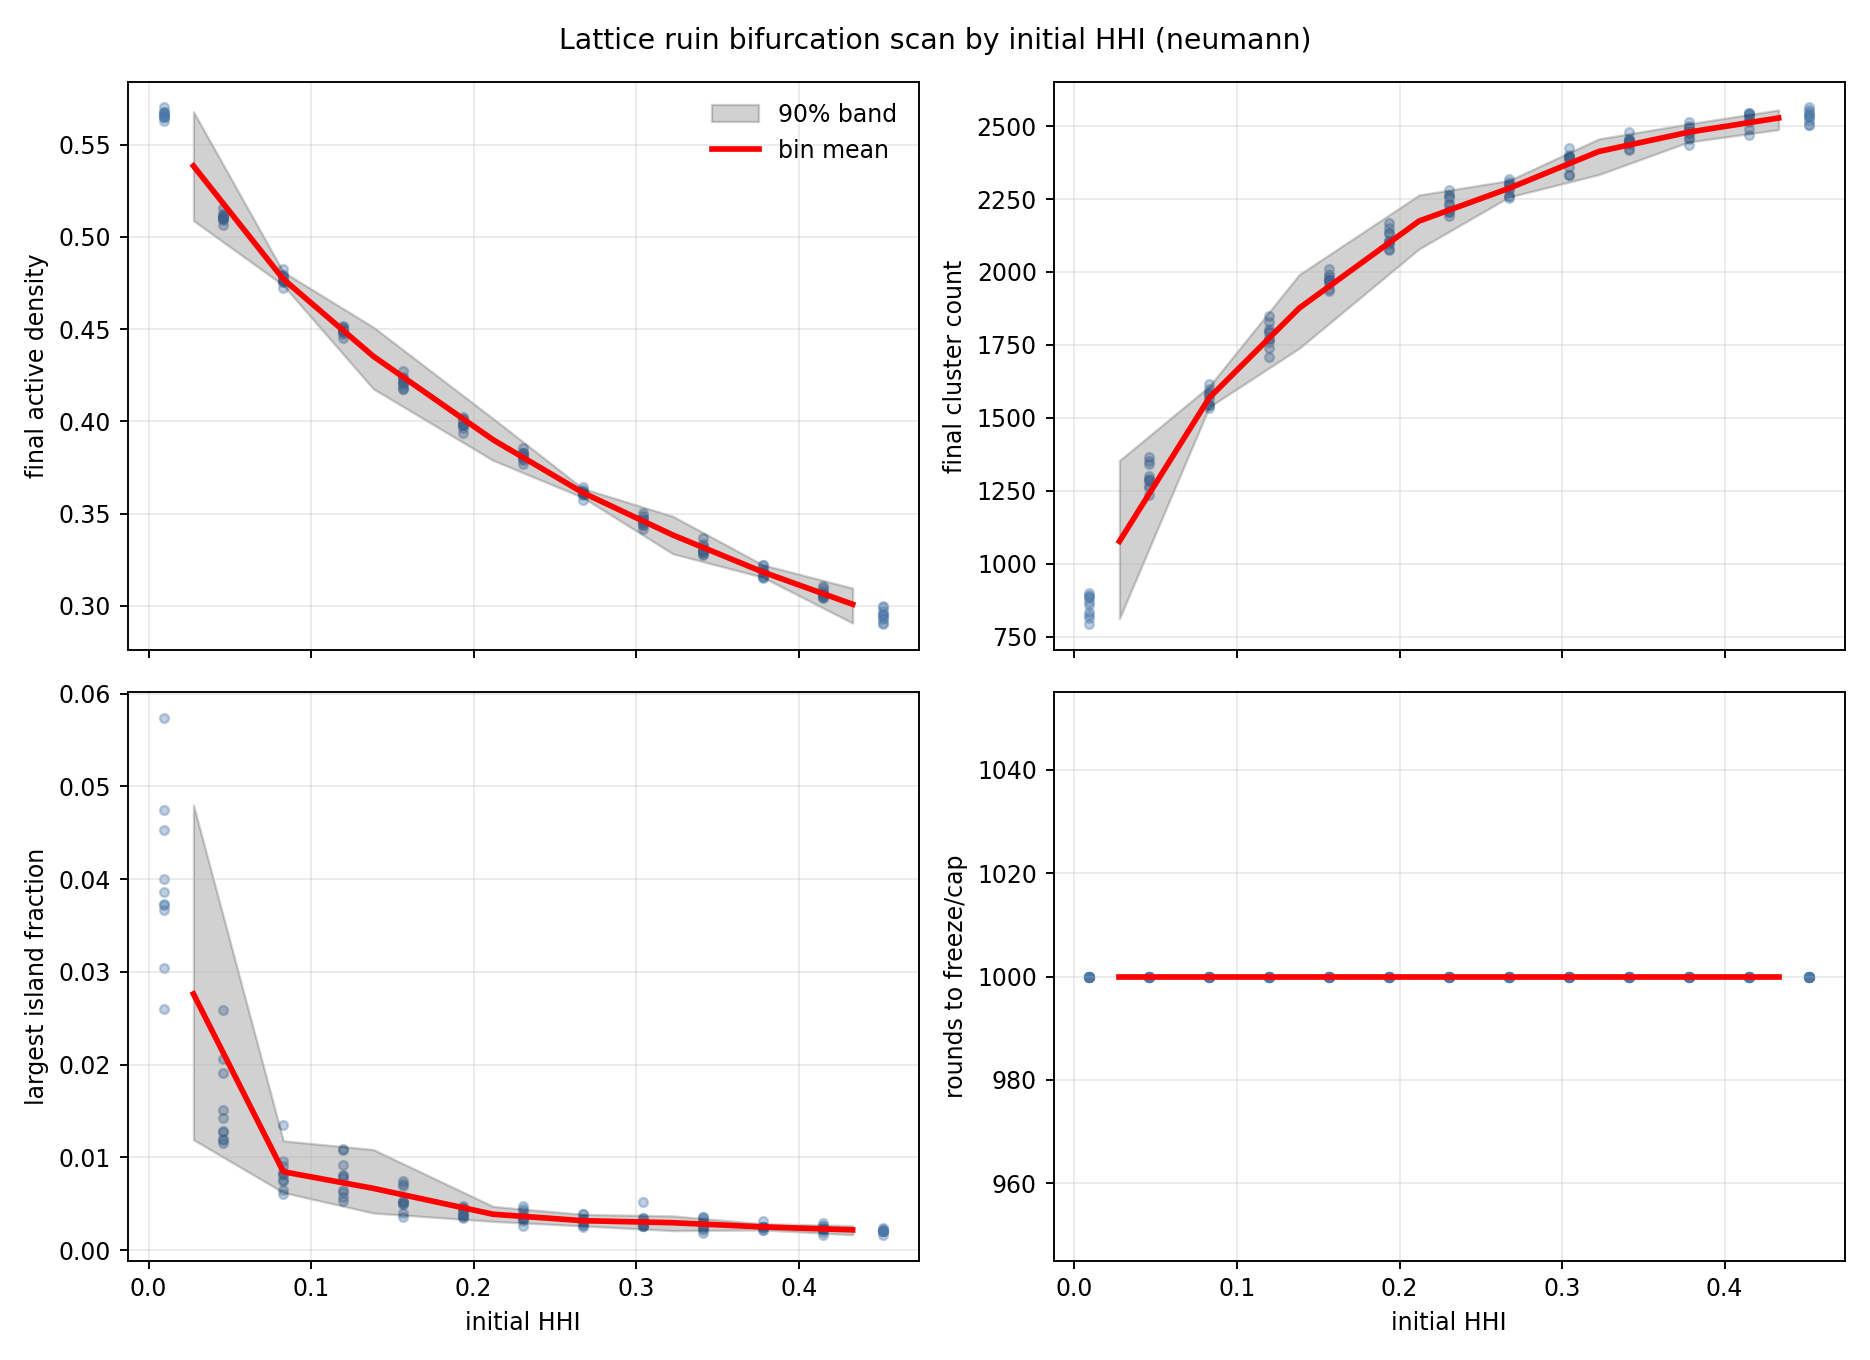
\includegraphics[width=0.96\linewidth]{figures/hhi_bifurcation_N100.png}
  \caption{Bifurcation-style scan using measured initial HHI. Points are individual simulations; red curves are binned means; black bands are 90\% intervals.}
  \label{fig:hhi}
\end{figure}

This is a useful bridge between the non-spatial and spatial problems. In the all-to-all gambler's ruin setting, concentration predicts absorption-time scale through pairwise wealth products and diversity. On the lattice, concentration also controls how much local interface is available for death-zone formation.

\subsection{Small-World Nonlocality}

The nonlocal scan is the cleanest new experiment. We add long-range edges while preserving the local lattice, then run each system without a round cap. Across $44$ values of $p$ and ten simulations per value, all $440$ runs froze and none globally absorbed. Thus, in this parameter regime, nonlocality does not restore the classical one-survivor outcome.

\begin{figure}[ht]
  \centering
  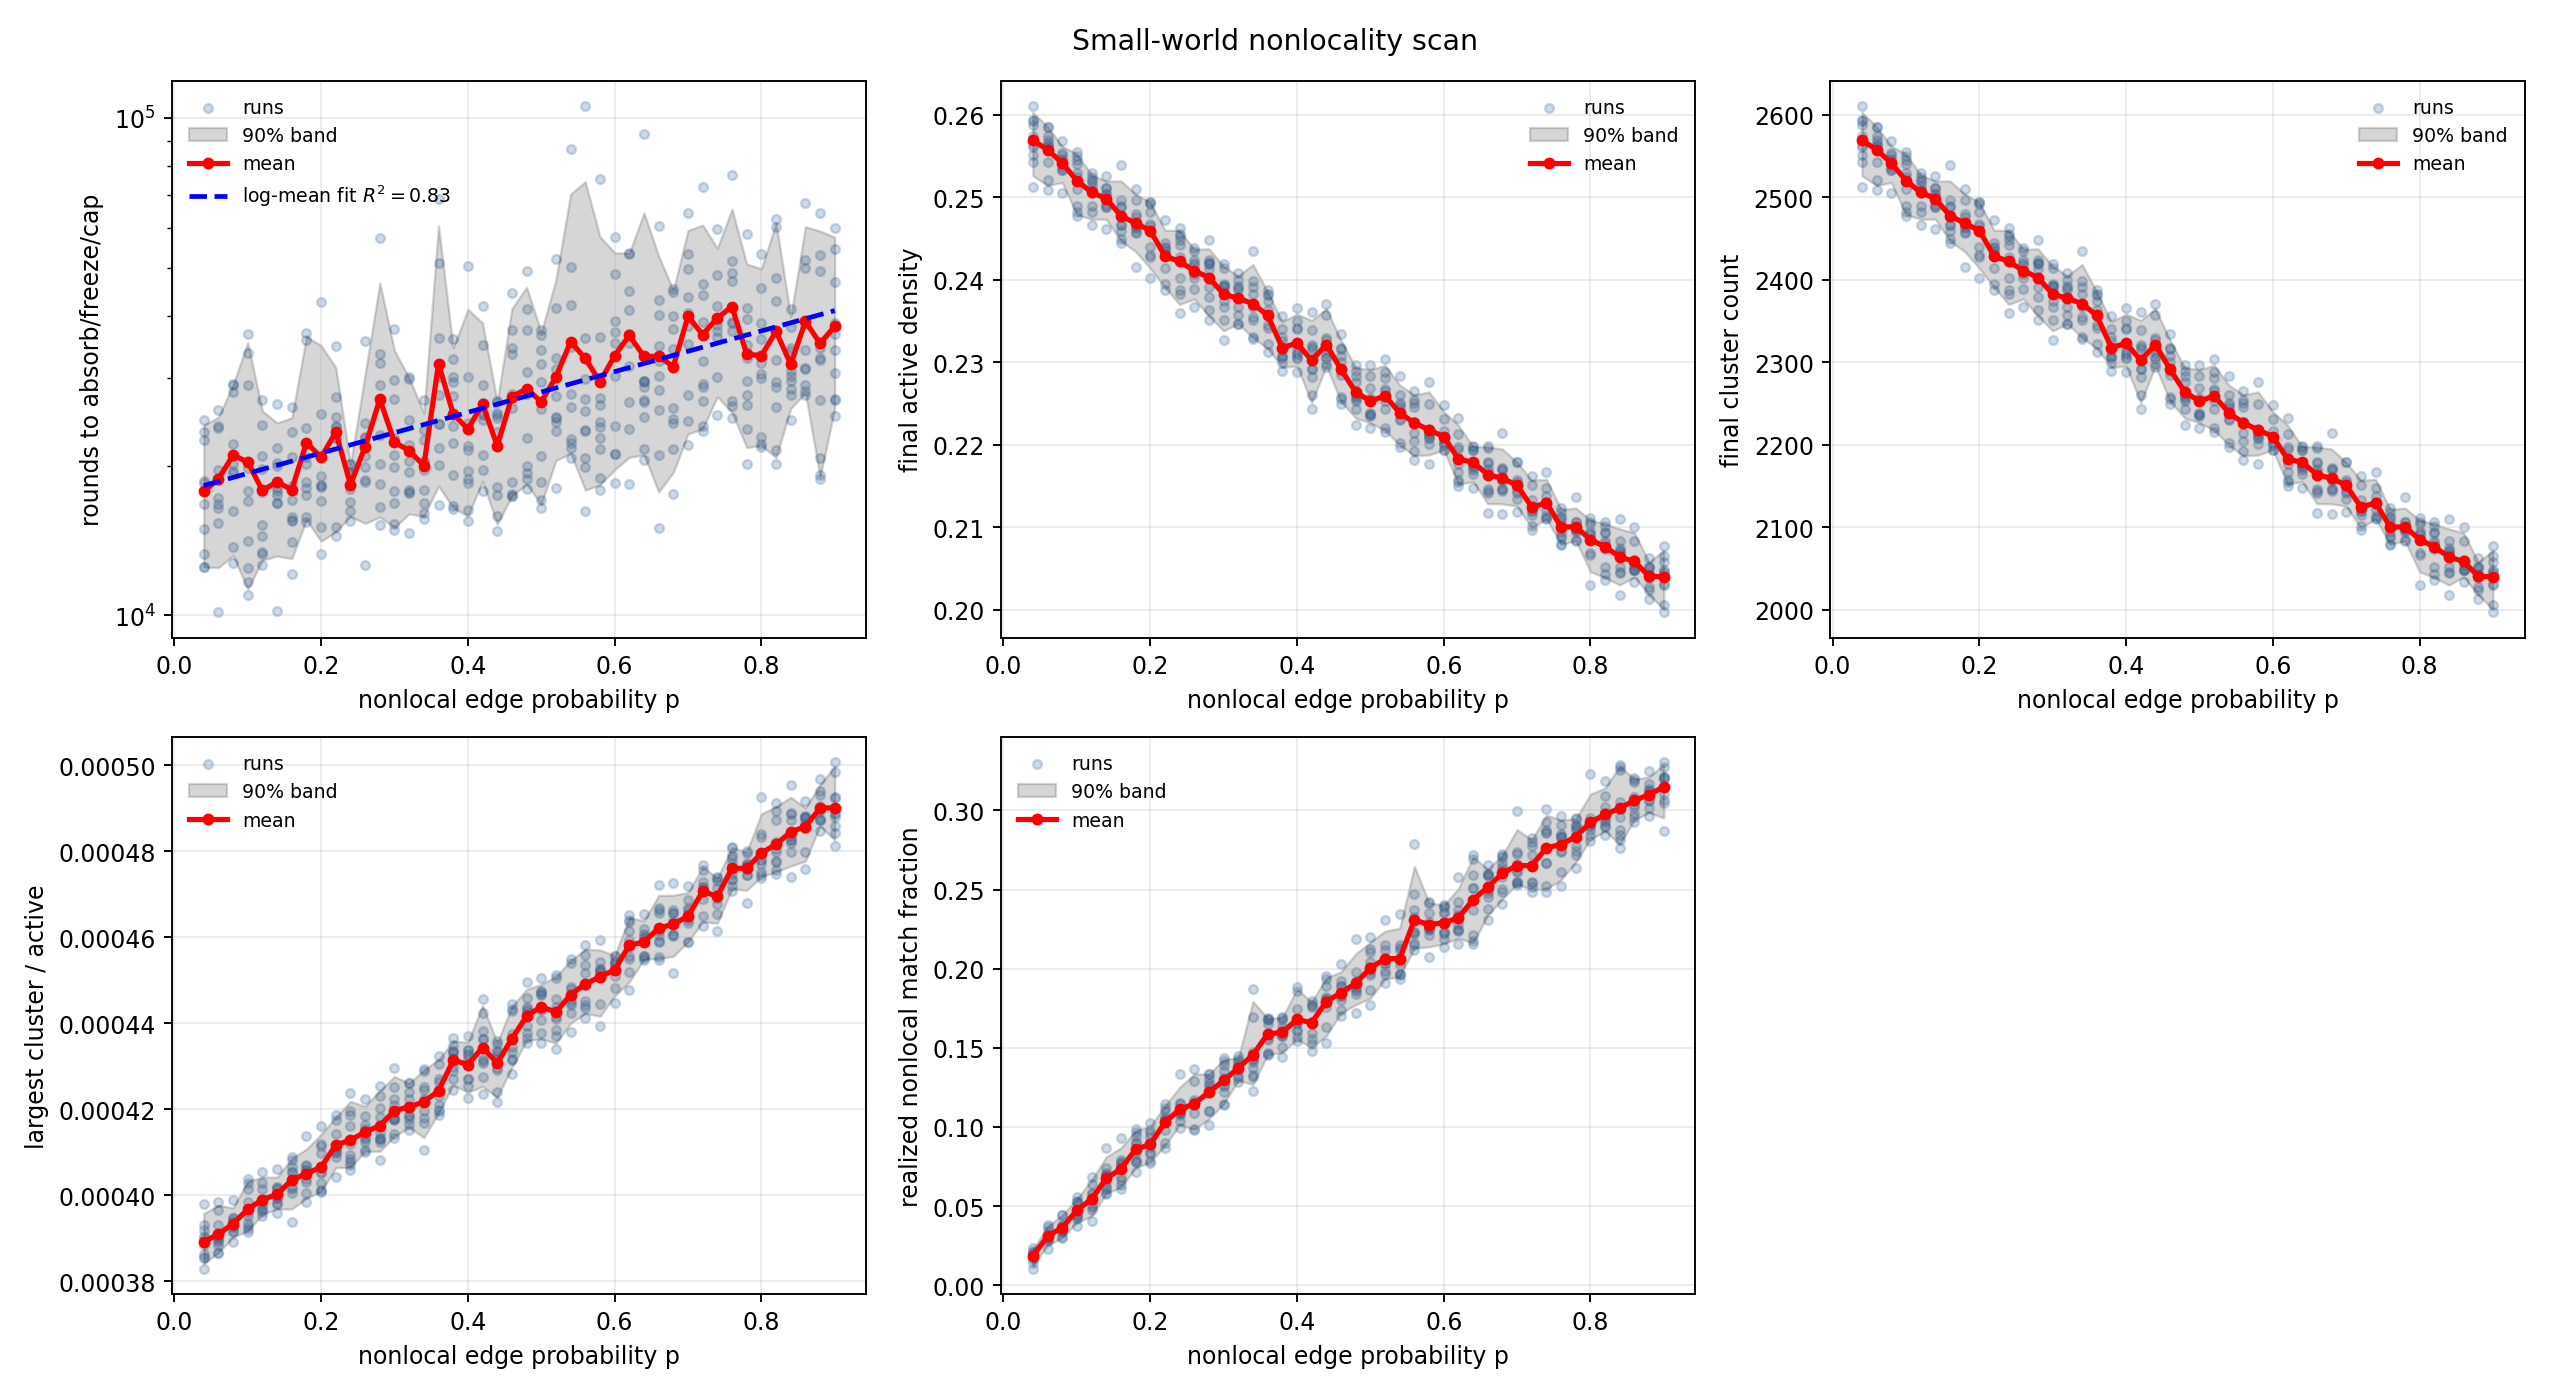
\includegraphics[width=0.96\linewidth]{figures/nonlocal_scan_N100_inw10_uncapped.png}
  \caption{Uncapped nonlocal scan, $N=100$, uniform initial wealth $10$, ten simulations per $p$. Increasing nonlocality lowers final active density and cluster count while increasing the realized fraction of nonlocal matches. Freeze time tends to increase.}
  \label{fig:nonlocal}
\end{figure}

\begin{table}[ht]
  \centering
  \caption{Selected mean values from the uncapped nonlocal scan. Every listed run froze; none was capped and none globally absorbed.}
  \begin{tabular}{rrrrrr}
\toprule
$p$ & Freeze time & Active density & Clusters & Nonlocal match frac. & Nonlocal edges \\
\midrule
0.04 & 17760 & 0.257 & 2569 & 0.018 & 395 \\
0.24 & 18323 & 0.242 & 2422 & 0.111 & 2412 \\
0.44 & 21902 & 0.232 & 2322 & 0.179 & 4378 \\
0.64 & 33161 & 0.218 & 2179 & 0.244 & 6389 \\
0.84 & 31976 & 0.206 & 2064 & 0.301 & 8406 \\
0.90 & 38124 & 0.204 & 2040 & 0.315 & 9012 \\
\bottomrule
\end{tabular}

  \label{tab:nonlocal}
\end{table}

The interpretation is subtle and important. Long-range edges give active sites more opportunities to keep gambling, so they prolong competition and eliminate more sites before the graph freezes. But the process still ends in an independent set of active survivors. Increasing $p$ from $0.04$ to $0.90$ lowers final active density from about $0.257$ to $0.204$, lowers final cluster count from about $2569$ to $2040$, and raises the realized nonlocal match fraction from about $0.018$ to $0.315$.

The largest-cluster fraction is not the headline metric in the fully frozen nonlocal runs. Since frozen active sites are isolated in the full interaction graph, the largest active cluster is usually size one. Therefore the ratio ``largest cluster / active sites'' can rise merely because the denominator shrinks. Active density, cluster count, freeze time, and realized nonlocal match fraction are the robust summaries.

\begin{figure}[ht]
  \centering
  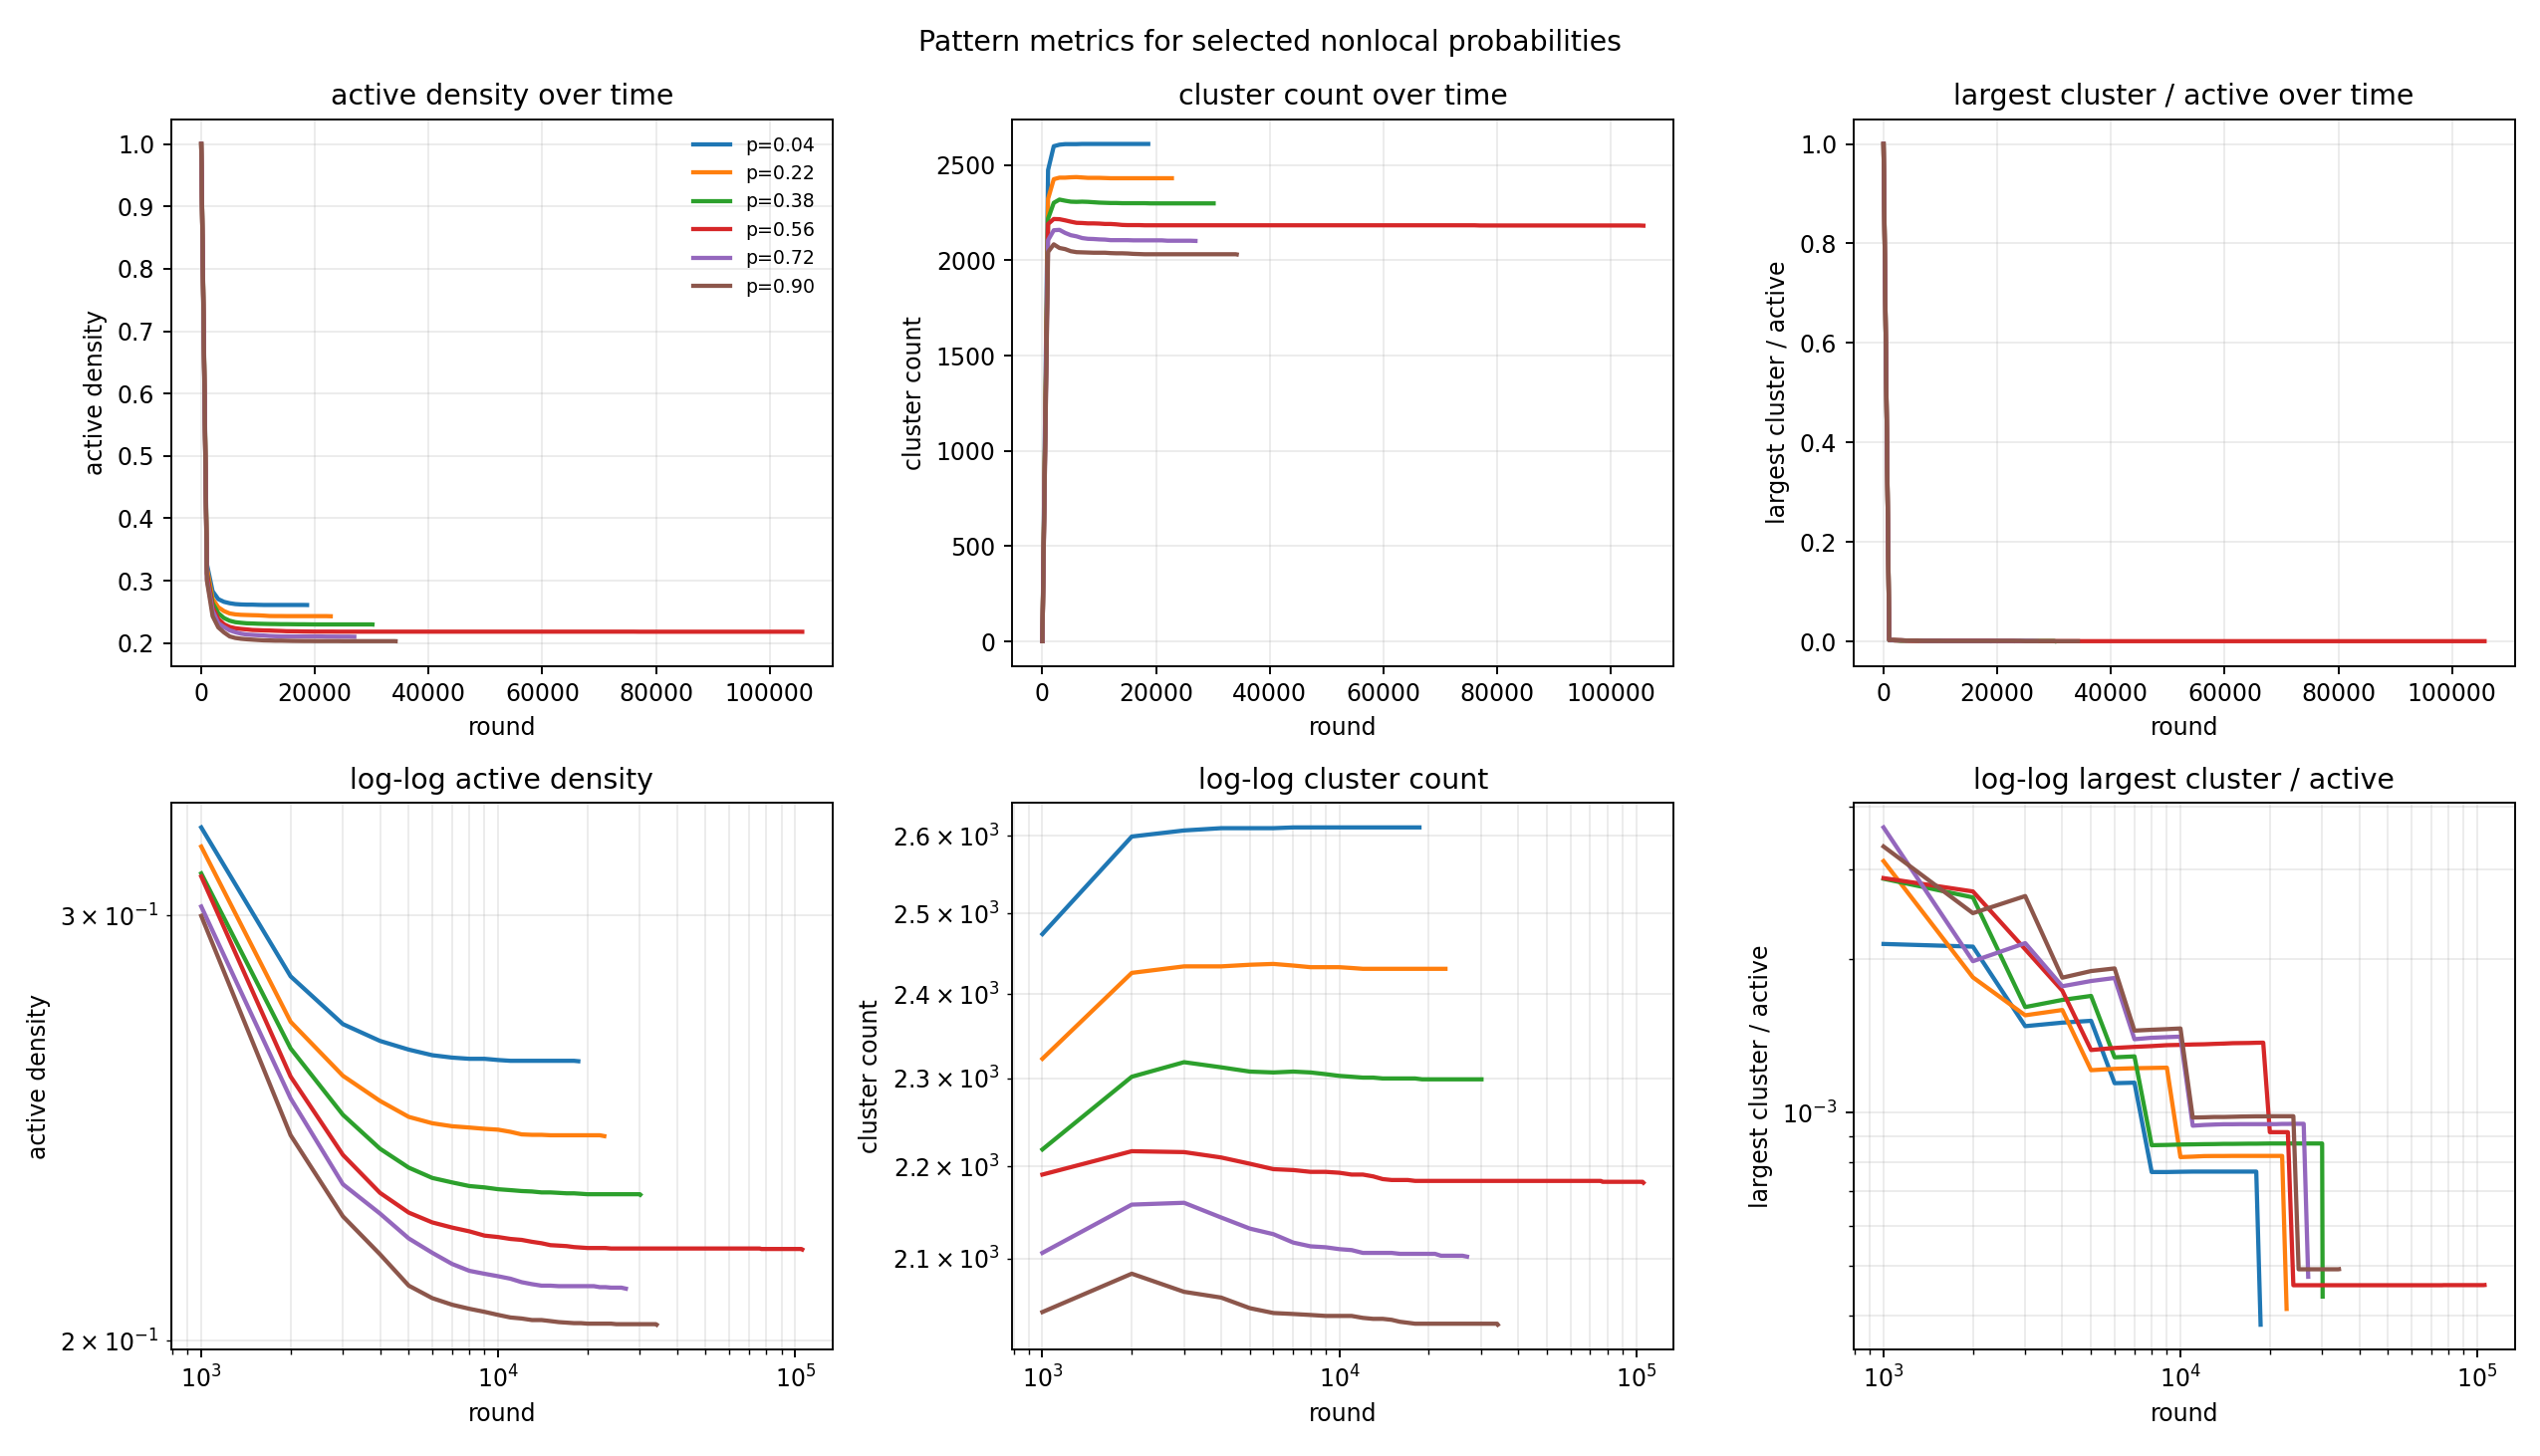
\includegraphics[width=0.96\linewidth]{figures/nonlocal_trajectories_N100_inw10_uncapped.png}
  \caption{Representative trajectories for selected nonlocal probabilities. Nonlocality accelerates the early density drop and extends the time over which residual active sites continue to interact.}
  \label{fig:nonlocal-trajectories}
\end{figure}

\section{Discussion}

The classical gambler's ruin intuition says that enough time creates one survivor. The lattice version shows why the phrase ``enough time'' depends on graph connectivity through the active subgraph, not merely on total wealth. Once dead barriers disconnect all active sites, the stochastic wealth exchange process has no legal move left. The absorbing object is therefore not a winner, but an independent active set.

This makes the model a compact pattern-formation laboratory. It has conservation, noise, irreversible death, and local geometry. Those ingredients are enough to produce dead zones, frozen islands, interfaces, fragmentation, and finite-time coarsening. The small-world experiment adds a useful negative result: more mixing need not imply one-winner absorption. In the tested regime, it produces longer competition and fewer survivors, but still freezes.

\section{Future Work}

The immediate next step is computational and theoretical. Computationally, the matching step should be optimized so larger uncapped scans can be repeated across neighborhoods, initial wealth scales, and periodic boundary conditions. Theoretically, the key object is the active graph process: death removes vertices, and the stopping state is an independent set of the evolving active graph. This suggests links to random sequential adsorption, percolation, voter-like coarsening, and absorbing-state phase transitions.

Several extensions are natural: Moore, triangular, and hexagonal neighborhoods; periodic lattices as finite approximations to infinite systems; weighted players with win probability $w_i/(w_i+w_j)$; and dynamic nonlocality where long-range edges appear transiently rather than statically. The empirical question is whether any of these variants creates a genuine transition between frozen-island absorption and global winner absorption.

\section{Conclusion}

The lattice gambler's ruin model turns a familiar martingale absorption problem into a spatial freezing problem. Initial wealth concentration shapes the emerging pattern, cluster-size plots reveal finite-time fragmentation, and nonlocal shortcuts intensify competition without eliminating frozen islands in the $N=100$, initial-wealth $10$ scan. The core message is simple: in spatial gambler's ruin with dead barriers, ruin does not just choose a winner; it writes a pattern into the graph.

\end{document}
